\chapter{Toolchain} \label{chap:toolchain}

The overall idea on how to achieve a toolchain that fully supports the requirements described in section \ref{sec:requirements} and to supports the modeler in the modeling process is, to develop an integrated development environment like they are used in computer sciences and software development. IDE’s, such as the well known Eclipse IDE, Netbeans or MS Visual Studio  are a very common and crucial tools in the area of software development. They provide the software developer with a set of very useful tools and functionality such as code completion, syntax highlighting, debugging features and so on. All of these tools allow the software developer to manage much more complex software projects and increases its productivity. Based on the premiss that software developers are nothing else than “modeler of source code”, the similarity to the problems in the environmental modeling domain are obvious. This chapter tries to outline the idea of such a specialized IDE for environmental modeling. In order to do this, we decided to describe a workflow including the steps a modeller has to take, to define a model with such an IDE.


A very extensive discussion of a modeling process can be found in \autocite{Jakeman2006602}. Hence this article targets the quality of the model process itself and does not take into account how this workflow can be supported by tools, we decided to take a much more simpler modelling workflow that is more suitable and based on the steps necessary using an IDE for the modelling process.Picture \ref{fig:modeling_workflow} depicts this simplified modeling workflow.
%TODO insert picture
%\begin{figure}[h]
%	\centering
%	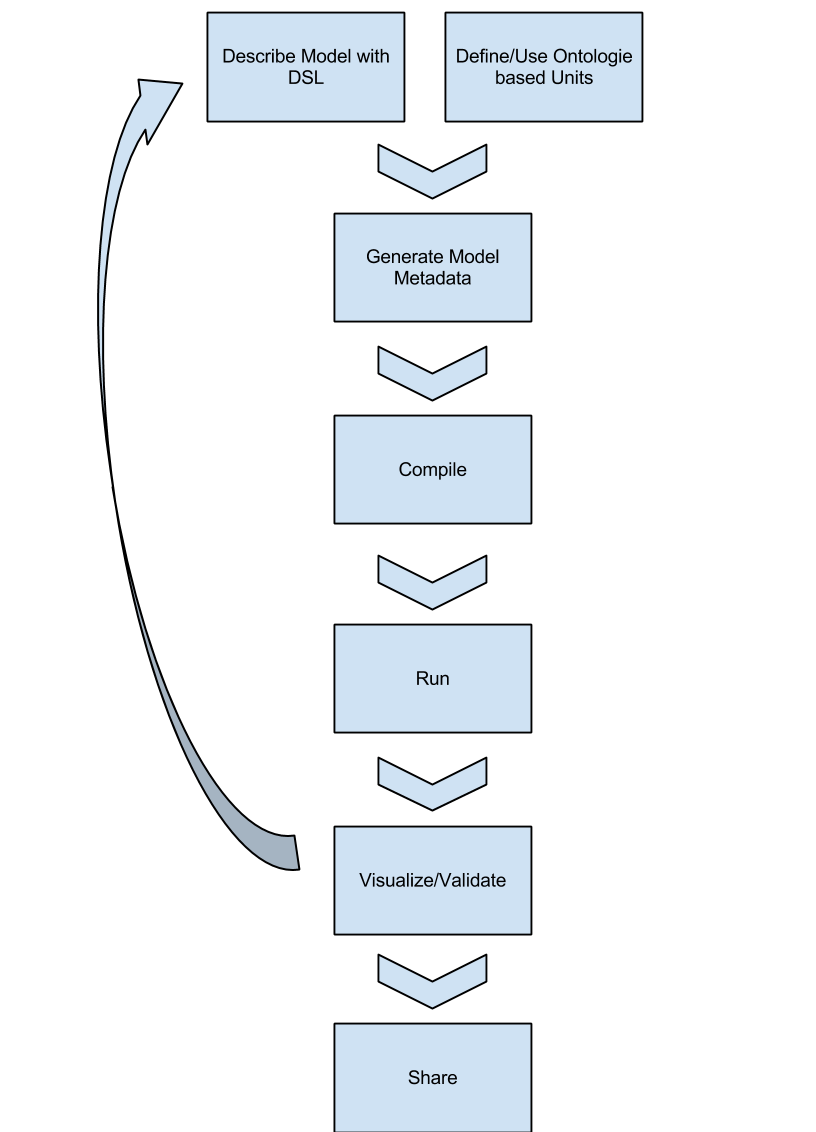
\includegraphics[width=0.7\textwidth]{pics/toolchain/modeling_workflow.png}
%	\caption{modeling workflow \label{fig:modeling_workflow}	
%\end{figure}


We decided to start with the implementation of the model. Prior steps such as defining the model purpose, specifying model context and so on, like they are recommended in \autocite{Jakeman2006602} are left out intentionally in fact we want to emphasize the use of the IDE and to concentrate on the requirements derived from chapter \ref{sec:requirements}. In the following sections we want to explain the different steps and what features the IDE can offer to support the user in more detail. 


\section{Writing a model}
The modeler starts with the implementation/coding of the model. Since this is the most basic part of the IDE and the main interface for the user, this is the place to include the most relevant and crucial tools to support the user during the coding phase. These features are very diverse and range from very simple and basic ones like code completion, syntax highlighting, automatic warnings and action items to much more complex and specialized ones that belongs to the requirements from chapter \ref{sec:requirements}. One of these very specific features are domain specific semantic datatypes and the handling of typical operations as explained earlier. In order to achieve these features, it is necessary to define important semantical aspects of entities and datatypes used in the model.


A very common approach to define the semantics in a formal and machine readable way (which is important for later code generation) are ontologies (see \nameref{sec:app:ontology} for an short explanation of ontologies). The reasons for this are discussed in[literature research paper das das belegt]. And also in the environmental domain ontologies are often used and are a very common way to define semantics of entities. \autocite{dsl:muetzelfeldt}, \autocite{Villa2009577}


Therefore the semantics of every used entity or datatype must be defined in an ontology which then can be used to automatically check consistency of the model, and that allows the IDE to handle typical operations like automatic unit conversions. Actually there are a set of projects that has focused on this topic  and that developed a set of ontologies that define the semantic of entities in the environmental domain.  QUDT, which stands for Quantities, Units, Dimensions and Data Types in OWL and XML [2] is one of these projects and one of it’s goals is to “to provide a unified model of, measurable quantities, units for measuring different kinds of quantities, the numerical values of quantities in different units of measure and the data structures and data types used to store and manipulate these objects in software” [2]. Another, more famous project is Nasa SWEET [3] (Semantic Web for Earth and Environment Technologies) which provides a very extensive set of ontologies and “include several thousand terms, spanning a broad extent of Earth system science and related concepts”[4]
A very common approach to define the semantics in a formal and machine readable way (which is important for later code generation) are ontologies (see Appendix XX for an short explanation of ontologies). The reasons for this are discussed in[literature research paper das das belegt]. And also in the environmental domain ontologies are often used and are a very common way to define semantics of entities. [muetzelfeld paper, als beleg, ioannis paper als beleg] 


Therefore the semantics of every used entity or datatype must be defined in an ontology which then can be used to automatically check consistency of the model, and that allows the IDE to handle typical operations like automatic unit conversions. Actually there are a set of projects that has focused on this topic  and that developed a set of ontologies that define the semantic of entities in the environmental domain.  QUDT, which stands for Quantities, Units, Dimensions and Data Types in OWL and XML [2] is one of these projects and one of it’s goals is to “to provide a unified model of, measurable quantities, units for measuring different kinds of quantities, the numerical values of quantities in different units of measure and the data structures and data types used to store and manipulate these objects in software” [2]. Another, more famous project is Nasa SWEET [3] (Semantic Web for Earth and Environment Technologies) which provides a very extensive set of ontologies and “include several thousand terms, spanning a broad extent of Earth system science and related concepts”[4]

